\documentclass{article}
\usepackage{graphicx}

\title{Sprawozdanie z laboratorium nr 2 z Technik Programowania Rownolegleglo}
\author{Jakub Janczak}

\begin{document}
\maketitle
\section{Wyliczanie liczby PI}

Wyliczanie liczby PI przeprowadzamy z pomoca algorytmu polegajacego na losowaniu punktow z z przedzialu (0,1) i sprawdzania czy para (x,y) znajduje sie w kole o promieniu r=1/2 i srodku w pkcie (0.5,0.5).

Wykres bledu wzglednego w st do liczby iteracji

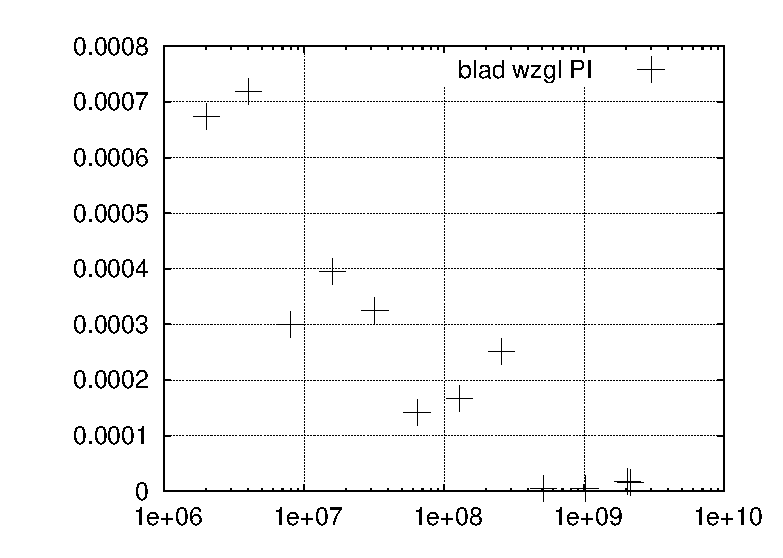
\includegraphics{wzgl.eps}

Wykres bledu bezwzglednego w st do liczby iteracji

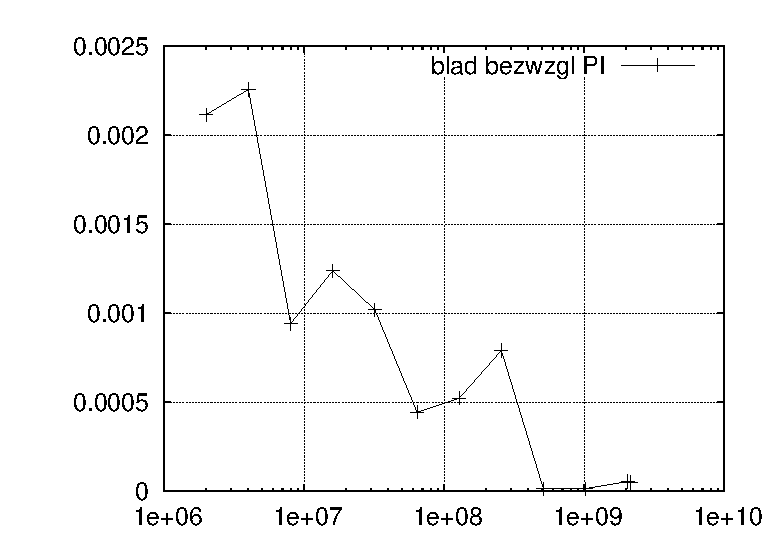
\includegraphics{bezwzgl.eps}

\subsection{Przyspieszenie(speedup)} - jest to czas w jakim program wykonuje sie sekwecyjnie w stosunku do czasu w jakim program wykonal sie rownolegle
\( S(n) = T(1) / T(n) \)
Wykres przyspieszenia dla problemu

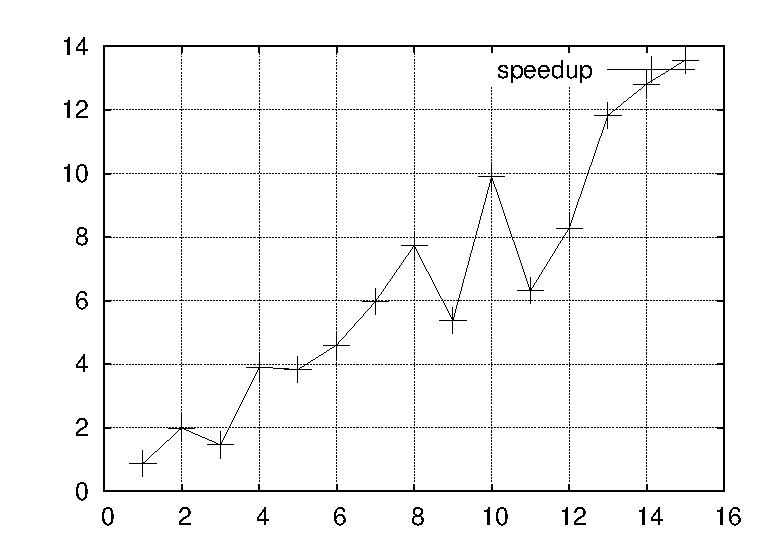
\includegraphics{speedup.eps}

\subsection{Przyspieszenie skalowalne} - to przyspieszenie ktore mierzymy proporcjonalnie ze wzrostem wielkosci problemu 

Wykres przyspieszenia skalowalnego dla problemu

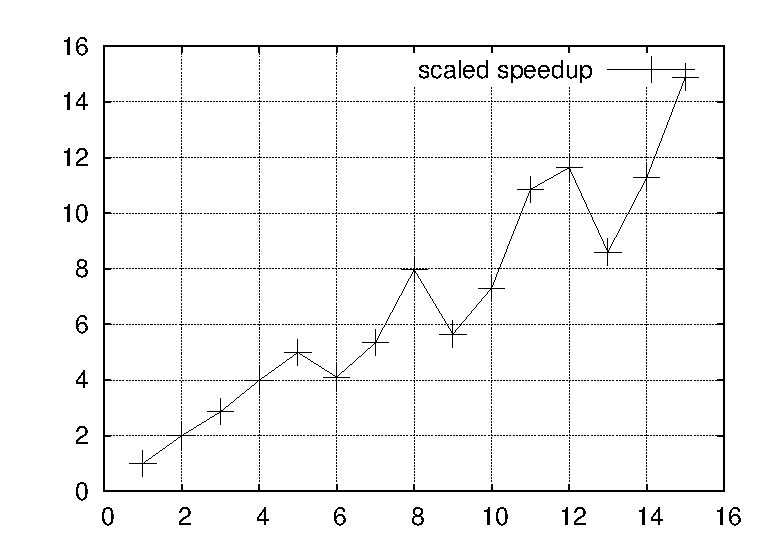
\includegraphics{speedup_sc.eps}

\subsection{Efektywnosc}  - jest to wartosc przyspieszenia w stosunku do ilosci uzytych do obliczenia procesorow.
Wykres efektywnosci dla problemu

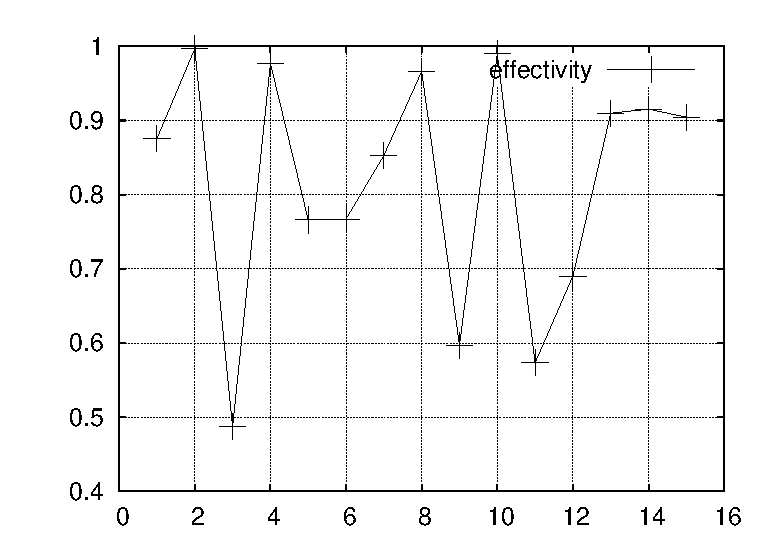
\includegraphics{effect.eps}

\subsection{Efektywnosc skalowalna}
mierzona jest z proporcjonalnym wzrostem wielkosci problemu w stosunku do ilosci procesorow
Wykres efektywnosci skalowalnej:

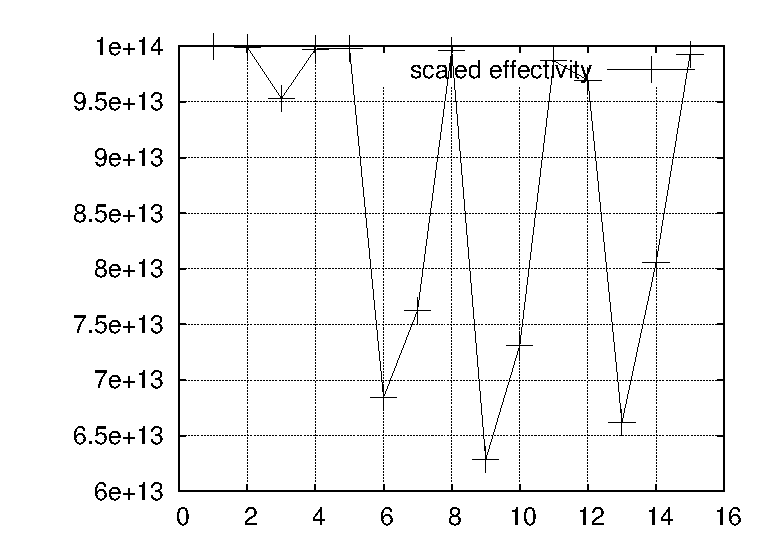
\includegraphics{effect_sc.eps}

\section{Rownolegle mnozenie macierzy}

Przeprowadzilem je stosujac najprostszy z mozliwych algorytmow tj. dla problemu
\( C = A*B \)
kazdemu z wezlow wysylam macierz B i dziele pomiedzy nie wiersze macierzy A. W odpowiedzi master otrzymuje przemnozone wezly macierzy C. Obliczen dokonalem z pominieciem narzutu komunikacyjnego-jego udzial w tym algorytmie jest bardzo znaczacy.

\subsection{Przyspieszenie}

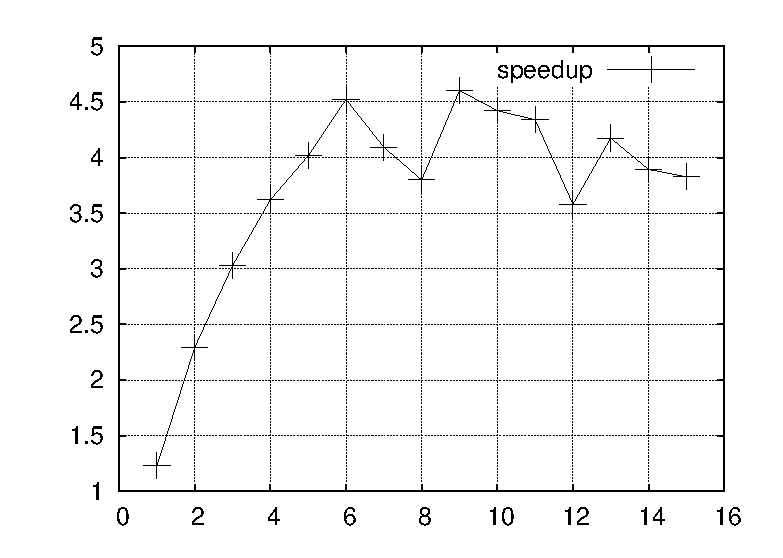
\includegraphics{speedup1.eps}

\subsection{Przyspieszenie skalowalne}

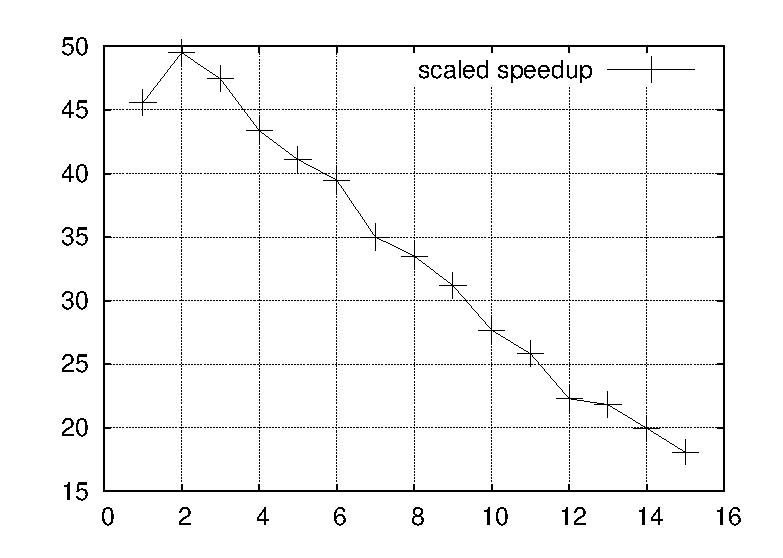
\includegraphics{speedup1_sc.eps}

\subsection{Efektywnosc}

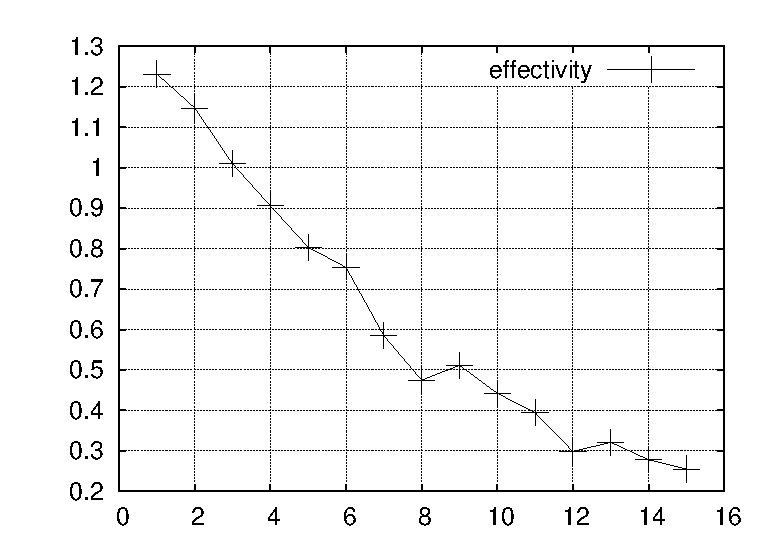
\includegraphics{effect1.eps}

\subsection{Efektywnosc skalowalna}

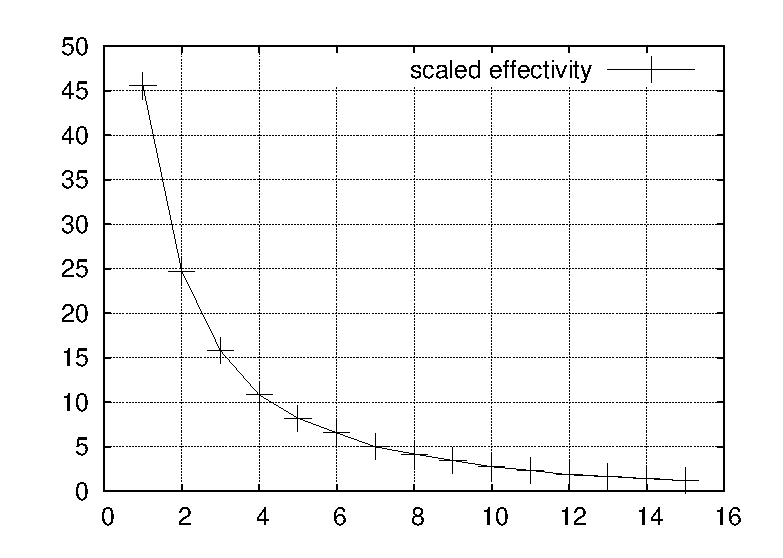
\includegraphics{effect1_sc.eps}


\subsection{Mnozenie z wykorzystaniem struktury hypercube}
Dodatkowo chcialem pokazac umieszczony w przykladach ciekawy algorytm korzystajacy z obracania wierszy, ale niestety nie dzialal on na udostepnionej maszynie ;(
\end{document}
